%%% Template for documenting projects which involve circuit illustrations and code.
% Author: Claudiu Groza

% Template based on the template created by:
% Author:   Luis José Salazar-Serrano
%           totesalaz@gmail.com / luis-jose.salazar@icfo.es
%           http://opensourcelab.salazarserrano.com


\documentclass[a4paper,11pt]{article}

\usepackage[T1]{fontenc}
\usepackage[utf8]{inputenc}
\usepackage{graphicx}
\usepackage{xcolor}

\renewcommand\familydefault{\sfdefault}
\usepackage{tgheros}
\usepackage[defaultmono]{droidmono}

\usepackage{amsmath,amssymb,amsthm,textcomp}
\usepackage{enumerate}
\usepackage{multicol}
\usepackage{tikz}
\usepackage{courier}

\usepackage{pythonhighlight}

\usepackage{hyperref}

\usepackage{geometry}
\geometry{total={210mm,297mm},
left=25mm,right=25mm,%
bindingoffset=0mm, top=20mm,bottom=20mm}


\linespread{1.3}

\newcommand{\divider}{\rule{\linewidth}{0.5pt}}

% my own titles
\makeatletter
\renewcommand{\maketitle}{
\begin{center}
\vspace{2ex}
{\huge \textsc{\@title}}
\vspace{1ex}
\\
\divider\\
\@author \hfill \@date
\vspace{4ex}
\end{center}
}
\makeatother
%%%

% custom footers and headers
\usepackage{fancyhdr}
\pagestyle{fancy}
\lhead{}
\chead{}
\rhead{}
\lfoot{Fire Fighter Car System}
\cfoot{}
\rfoot{Page \thepage}
\renewcommand{\headrulewidth}{0pt}
\renewcommand{\footrulewidth}{0pt}
%

% code listing settings
\usepackage{listings}

\lstset{%
  language = Octave,
  backgroundcolor=\color{white},   
  basicstyle=\footnotesize\ttfamily,       
  breakatwhitespace=false,         
  breaklines=true,                 
  captionpos=b,                   
  commentstyle=\color{gray},    
  deletekeywords={...},           
  escapeinside={\%*}{*)},          
  extendedchars=true,              
  frame=single,                    
  keepspaces=true,                 
  keywordstyle=\color{orange},       
  morekeywords={*,...},            
  numbers=left,                    
  numbersep=5pt,                   
  numberstyle=\footnotesize\color{gray}, 
  rulecolor=\color{black},         
  rulesepcolor=\color{blue},
  showspaces=false,                
  showstringspaces=false,          
  showtabs=false,                  
  stepnumber=2,                    
  stringstyle=\color{orange},    
  tabsize=2,                       
  title=\lstname,
  emphstyle=\bfseries\color{blue}%  style for emph={} 
} 

%%%----------%%%----------%%%----------%%%----------%%%

\begin{document}

\title{Fire Fighter Car System}

\author{Alexandra Ciobotea, Daian Stein, Politehnica University of Timisoara}

\date{June, 2018}

\maketitle


\section{Repository}
\text{The project history, schematics, diagrams and codebase are contained under the following git repository:}\\
\textbf{\url{https://github.com/steindaian/FireFighterCar}}

\section{User requirements}

\begin{enumerate}  
\item The system provides information about the environment conditions, as the car is meant to be used as a tool for emergency situations such as CO leak.
\item The system is equiped with humidity, temperature, proximity and CO detection sensors.
\item The tool provides a live video stream which is broadcasted to a controller application.
\item All the environment information are stored in a cloud storage system and can be accessed via the Android application or directly from the WEB; the data is updated once in 10 seconds.
\end{enumerate}

\section{System overview}

The overview of the system is depicted in figure \ref{fig:system}.

\begin{figure}[h]
\centering
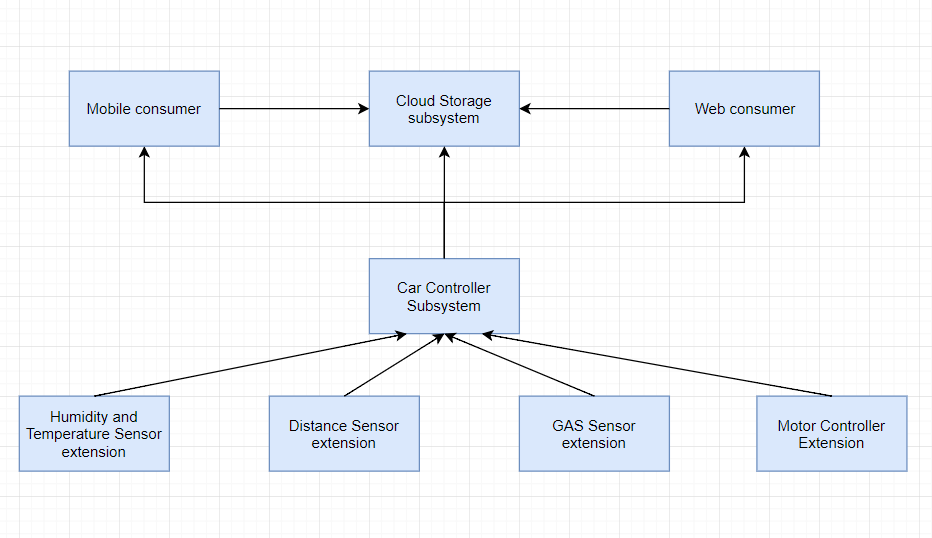
\includegraphics[scale=0.5]{overview.png}
\caption{System overview diagram}
\label{fig:system}
\end{figure}

Base (Car Controller) Subsystem encompasses the measurement functionality, the movement controll of the car and the video stream broadcasting. It has the sole purpose to acquire information from it’s sensors(Humidity,Temperature,CO,Distance-Proximity) and extensions.\\

The camera(the motion service) together with the engine controller form the Motor Controller Extension.\\

Cloud Storage Subsystem stores the data pushed by the Base Subsystem. Additionally, it offers a possibility to interpret stored information.\\

Web consumer provides the video stream depicted by the car's camera. This view is accessed within a Web browser.\\

Mobile application is in charge with car's movement. It also offer the posibility to analyze data from the Cloud and to visualise the live video stream from the car. The view will be accessed via a specialised application which runs on an Android device.

\section{Circuit design}

The hardware view of the system is depicted in figure \ref{fig:circuit-design}.

\begin{figure}[h]
\centering
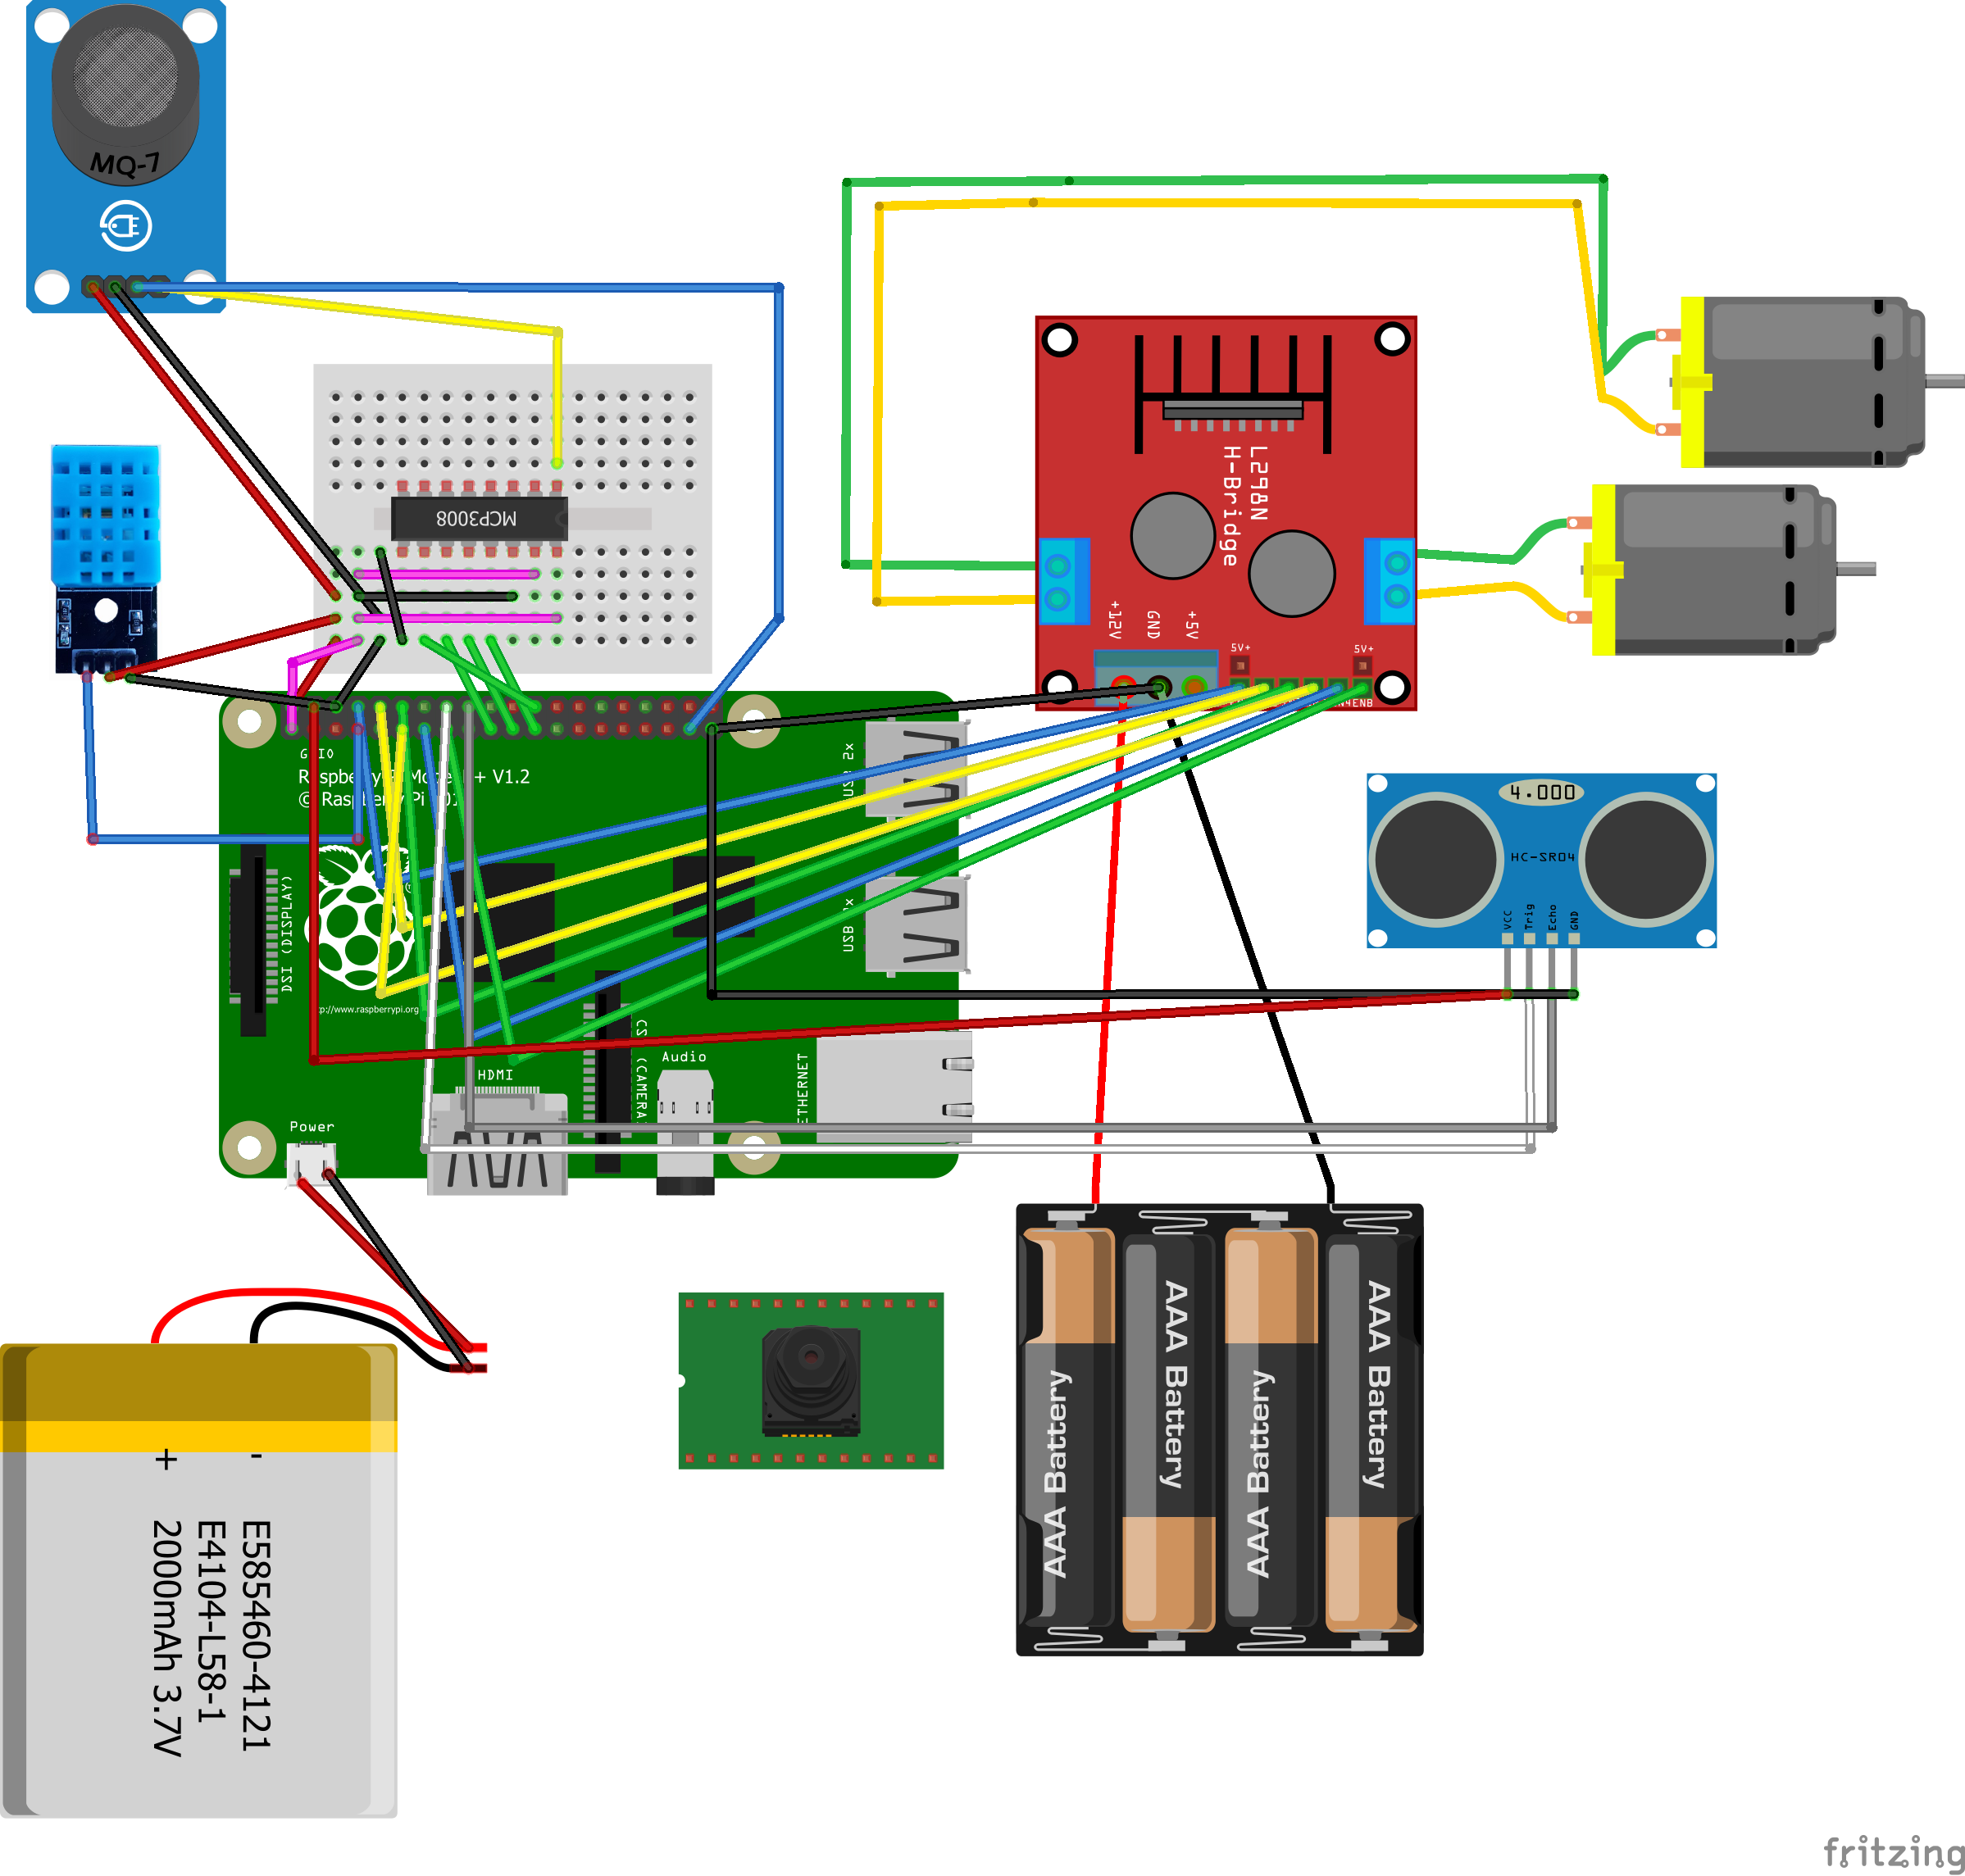
\includegraphics[scale=0.7]{hardware.png}
\caption{Circuit schematic}
\label{fig:circuit-design}
\end{figure}

Raspberry Pi 1 Model B+ provides support for quick prototyping. We will use the one-wire interface it has, but also the implicit possibility of communicating with other devices over the Internet. \\

For powering the board a 5000mAh power bank is used.\\

DHT-11 is an one-wire enabled sensor. It is a basic, digital-output relative temperature and humidity sensor.\\

CO detection sensor is an analogic sensor, which needs an analog-digital convertor(MCP3008) to gather the values properly. For the communication between the convertor and the Pi the SPI protocol was used.\\

The distance-proximty sensor(an ultrasonic sensor) is a digital component, used for rounding the up-front obstacles.\\

One of the two engines depicted above is used for speed controlling, while the other one for steering. The battery socket and the motor driver shield offer the strength and precision of the whole car movement.\\

The system uses Raspberry Pi's Camera v1.\\


\section{Software design}

The software components and data flow directions are depicted in figure \ref{fig:soft-design}. Each of these will be presented in the following subsections.\\

\begin{figure}[h]
\centering
\includegraphics[scale=0.7]{software.png}
\caption{Software entities involved}
\label{fig:soft-design}
\end{figure}
 
\subsection{Python modules}

sensor.py: it retrieves the outside sensor values and then pushes it to Firebase every 10 seconds.\\

Adafruit\_DHT11 library: it provides a quick implementation of one-wire interface communication with the temperature and humidity sensor.\\

Adafruit\_MCP3008 library: it is used for properly reading the CO related sensor values. Together with mq.py library normalize data and saves them for later on.\\

read\_distance function is used for computing the distance from the up-front object, based on simple mathematical equation.\\

motor.py: it is the submodule responsible with setting the speed and the steering of the car. It uses the RPI.GPIO library for the fine controlling movements(PWM).\\

main.py: the whole system starts from this script. It uses the above modules and it starts the camera stream service. Also, it creates the server socket responsible for communication with the Controller Application.\\

\subsection{Firebase}
Firebase is a PaaS (Platform as a Service) which means it offers developers to a quick list of functionalities supported by a traditional backend.
Realtime Database simplifies storing and synchronising data between different devices in realtime using a noSQL database.

The following code section shows the initialization of the Firebase project.

\begin{python}
# the generated root for your project
FIREBASE_ROOT = 'https://ms-proj.firebaseio.com'
# init Firebase Database instance
firebase = firebase.FirebaseApplication(FIREBASE_ROOT, None)
\end{python}

\subsection{Android application}
The Android application represents the Controller part of the FireFighterCar. The application assumes that the car(Raspberry Pi) is connected to the same network as the application is.\\

The main features used for constructing this application are:
\begin{itemize} 
\item A WebView UI component for viewing the video feed streemed from raspberry(+additional camera data)
\item Two joystick-like buttons for controlling the steering and the speed of the car; the communication is taking place using socket services
\item A TextView with the sensor data from the car(using Firebase Realtime Database)
\item Speech to Text translation using SpeechRecognizer service provided by Google
\item Concurrent jobs, network-based discovery functions(for searching the Pi's IP) and other mechanism used for building a smooth Controller Application
\end{itemize}

\subsection{WEB client}

The Web Client offers a way to debug the video stream, without controlling the motors and cloud retrival information.\\


\section{Results and further work}

The current version of the project supports the following functionalities:
\begin{itemize}  
\item reliable reading of the data sensors
\item storing data to Firebase Realtime Database
\item a client implementations for retrieving data stored in Firebase Database (Android) and controlling the system
\item a way to debug the camera submodule using a simple Web Browser
\item a live video stream to the Controller subsystem
\item speech recognizer for ease of use(designed for industrial usage)
\end{itemize}

The following list of extensions and improvements was identified to be supported in the future:
\begin{itemize}  
\item the system may provide a module for data interpretation.
\item remote access for configuring data interval reading
\item extend car capabilities of interpreting the video stream(Human recognition)
\item improve the hierarchy design of Firebase Database
\item a way of centralizing sensor data and outputs frame from the camera(to be used by a supervisor in activity field)
\end{itemize}

\newpage
\section{References}
\begin{enumerate}
\item Draw IO [last seen: May 2018], \url{https://www.draw.io/}
\item Fritzing [last seen: May 2018], \url{http://fritzing.org/}
\item Firebase Database [last seen: May 2018], \url{https://firebase.google.com/docs/database/}
\item DHT11Datasheet [last seen: May 2018], \url{https://akizukidenshi.com/download/ds/aosong/DHT11.pdf}
\item AdafruitDHT library [last seen: May 2018], \url{https://github.com/adafruit/Adafruit\_Python\_DHT}
\item AdafruitMCP3008 library [last seen: May 2018], \url{https://github.com/adafruit/Adafruit\_Python\_MCP3008}
\item MQ-7 library [last seen: May 2018], \url{https://github.com/tutRPi/Raspberry-Pi-Gas-Sensor-MQ/blob/master/mq.py}
\item Android Devlopers Guide [last seen: May 2018], \url{https://developer.android.com/guide}
\item Motion Camera Service [last seen: May 2018], \url{http://www.lavrsen.dk/}
\item Virtual Joystick for Android [last seen: May 2018], \url{https://github.com/controlwear/virtual-joystick-android}
\end{enumerate}



\end{document}